\chapter{Implementación}
\label{chapter:implementacion}

Este capítulo describe en detalle cómo algunas de las soluciones surgidas en el diseño fueron codificadas para resolver los requerimientos del problema original.

A continuación se explican algunas de las funcionalidades más relevantes denotadas en la etapa de diseño.


\section{Servidor FuD-BOINC}
La implementación del servidor FuD-BOINC se llevó a cabo sobre el sistema operativo Linux por dos motivos: por un lado, porque FuD y sus dependencias solo soportaban este sistema, y por el otro, porque el servidor de BOINC debe correr bajo este sistema operativo\footnote{\url{http://www.spy-hill.com/help/boinc/Create_Project.html\#server}}. Asimismo, en todo momento se trató de escribir código portable utilizando las librerías estándares.

	\subsection{BoincClientsManager}
Para proporcionar la funcionalidad de manejar un único cliente, con el inicio del sistema se hace una sola registración de un \texttt{BoincClientProxy} el cual perdurará durante toda la ejecución del servidor. De ésto se encarga el método \texttt{boinc\_register\_client()} el cual es invocado por el método \texttt{post\_initialization()} dentro del constructor \texttt{JobManager} de la capa L2. El último método mencionado forma parte de la reimplementación de FuD detallada en la sección \ref{seccion:jobmanager:post:init} de este proyecto. 

A continuación se muestra el código de la función \texttt{boinc\_register\_client()}:

\newpage

\begin{lstlisting}[frame=shadowbox, language=c++, numbers=left, xleftmargin=8mm, framexleftmargin=20pt, basicstyle=\footnotesize, numberstyle=\footnotesize, captionpos=b, caption={Método \texttt{boinc\_register\_client()} de la clase \texttt{BoincClientsManager}}, label=listing:BoincClientsManager:register:client, backgroundcolor=\color{gris}, firstnumber=66, keywordstyle=\color{Blue}]
void BoincClientsManager::boinc_register_client()
{
    // Init the client_proxy.
    boinc_log_debug(std::string(``Registering BOINC with FuD.''));
    BoincClientProxy * client = new BoincClientProxy();
    client->set_concurrent_jobs(UNLIMITED_JOBS);
    // Register the unique client proxy.
    register_client(client);
}
\end{lstlisting}

Por otro lado, bastó con que el método \texttt{should\_resend\_job\_units()} retorne \texttt{false} para indicar que FuD no reenvíe las \texttt{JobUnits}; tarea llevada a cabo por BOINC.
	
	\subsection{BoincClientProxy}
Si bien la creación de objetos \texttt{BoincClientProxy} es controlada por \texttt{BoincClientsManager}, se optó por utilizar el patrón de diseño Singleton para \linebreak restringir la creación de objetos de esta clase con el fin de evitar que se le dé un uso incorrecto en futuras implementaciones.

Esta es la clase más importante de la capa de distribución del lado servidor ya que es quien toma contacto con el proyecto BOINC mediante una conexión directa a su base de datos. Por esta razón, el constructor es el encargado de leer el archivo de configuración del proyecto BOINC (ver sección \ref{seccion:boinc:config:xml}) y de iniciar la conexión con la base de datos.

A continuación se muestra la implementación del constructor de la clase \texttt{BoincClientProxy}:

\begin{lstlisting}[frame=shadowbox, language=C++, numbers=left, xleftmargin=8mm, framexleftmargin=22pt, basicstyle=\scriptsize, numberstyle=\footnotesize, breaklines=true, breakatwhitespace=false, captionpos=b, caption={Constructor \texttt{BoincClientProxy}}, label=listing:BoincClientProxy, backgroundcolor=\color{gris}, firstnumber=83, keywordstyle=\color{Blue}]
BoincClientsManager::BoincClientProxy::BoincClientProxy() :
    ClientProxy(),
    _running_assimilator(true),
    raii_assimilator_db(db_assimilator),
    db_conn(boinc_db)
{
    set_log_level(LOG_HIGH);
    boinc_log_debug(std::string(``Parsing the BOINC config file.''));
    
    // Read the BOINC config file.
    int retval = config.parse_file();
    if (retval != RETVAL_OK)
    {
        std::string message =  ``Can`t parse BOINC config.xml file, '';
        message += boincerror(retval);
        throw (BoincFileException(message));
    }

    // Open the BOINC database.
    boinc_log_debug(std::string(``Connecting with the BOINC database.''));
    retval = boinc_db.open(config.db_name, config.db_host, config.db_user, config.db_passwd);
    if (retval != RETVAL_OK)
    {
        std::string message = ``Can`t open DB, '';
        message += boincerror(retval);
        throw (BoincDataBaseException(message));
    }

    //Creates assimilator thread to handle client response.
    _assimilator_thread = boost::thread( boost::bind( &BoincClientProxy::assimilator_thread, this ) );
}
\end{lstlisting}

La línea número 112 es la encargada de lanzar un nuevo hilo de ejecución el cual tiene como función notificar a la capa L2 los resultados recibidos por parte de los nodos de procesamiento. La sección \ref{seccion:asimilador} explica con más detalles la responsabilidad de este thread.

Otra de las funciones de esta clase es la de implementar el método \texttt{process()} provisto por FuD el cual es el encargado de enviar la \texttt{JobUnit} a un cliente. En este caso, la implementación de este método se encarga de serializar la \texttt{JobUnit} dentro de un archivo binario el cual va a ser utilizado para crear la \texttt{workunit} de BOINC. Toda esta funcionalidad a su vez se encuentra encapsulada dentro del método \texttt{boinc\_process()} el cual se describe a continuación:

\begin{lstlisting}[frame=shadowbox, language=C++, numbers=left, xleftmargin=8mm, framexleftmargin=22pt, basicstyle=\scriptsize, numberstyle=\footnotesize, breaklines=true, breakatwhitespace=false, captionpos=b, caption={Método \texttt{boinc\_process()} de \texttt{BoincClientProxy}}, label=listing:BoincClientProxy:boinc:process, backgroundcolor=\color{gris}, firstnumber=247, keywordstyle=\color{Blue}]
void BoincClientsManager::BoincClientProxy::boinc_process(const JobUnit& job_unit) 
                    throw(std::ofstream::failure, BoincAppException, BoincFileException, BoincWorkException )
{
    std::string name_input_file;
    generate_download_file(job_unit,name_input_file);

    // Read the wu_template.
    boinc_log_debug(std::string(``Reading the workunit template file''));
    char* wu_template;
    const int retval = read_file_malloc(config.project_path(WU_TEMPLATE.c_str()), wu_template);
    if (retval != RETVAL_OK)
    {
        std::string  description = ``Error in read_file_malloc, '';
        description += boincerror(retval);
        throw (BoincFileException(description));
    }

    create_boinc_work(name_input_file, wu_template);
}
\end{lstlisting}

El método invocado en la línea 251 es el encargado de crear el archivo binario con la información de la \texttt{JobUnit} dentro del directorio de descarga del proyecto para que los voluntarios lo descarguen cuando se le asigne la tarea asociada. En la línea 256 se lee la plantilla utilizada por BOINC en donde se especifica ciertas características que debe poseer la \texttt{workunit} a crear. Por último, en la línea 264 se lleva a cabo la creación de la \texttt{workunit} por medio de la invocación al método \texttt{create\_boinc\_work()}.

La implementación del método \texttt{create\_boinc\_work(std::string name\_input\_file, const char* wu\_template)} se puede simplificar en los siguientes pasos:

\begin{enumerate}
\item crear el nombre identificatorio de la \texttt{workunit},
\item obtener desde la base de datos la información de la aplicación asociada a esta tarea,
\item crear la \texttt{workunit} utilizando el nombre creado en el punto 1, la información de la aplicación obtenida en el punto 2, el archivo binario conteniendo la información de la \texttt{JobUnit} y la plantilla obtenida en la línea 256 del código  \ref{listing:BoincClientProxy:boinc:process} mencionada anteriormente. Para realizar este proceso se utiliza el método \texttt{create\_work()} provisto por BOINC\footnote{\url{http://boinc.berkeley.edu/trac/wiki/JobSubmission\#cpp-workgen}}.
\end{enumerate}

Por el contrario, la clase también se encarga de recuperar de la base de datos los resultados de las tareas enviadas. Para ello, se hizo la implementación de un asimilador de resultados.

	\subsubsection{Asimilador}
	\label{seccion:asimilador}
Una parte importante de la implementación de la clase \texttt{BoincClientProxy} consistió en poder integrar el comportamiento del demonio \textit{assimilator} (\ref{boinc:assimilator}) de BOINC como parte del comportamiento de esta clase al momento de manejar un resultado recibido desde el cliente. Debió realizarse esta integración ya que la manera en que BOINC propone la implementación de este demonio obliga a crear un nuevo ejecutable de manera independiente a la aplicación de FuD. Ésto evitaba respetar el modelo de FuD, en donde la misma aplicación debe encargarse de atrapar e interpretar los resultados de las tareas concluidas.

Por ello, el asimilador se implementa en un nuevo hilo de ejecución, utilizando \texttt{boost::thread}\footnote{\url{http://www.boost.org/}}, dentro del servidor FuD-BOINC encargándose de chequear la existencia de resultados no asimilados. Si la unidad de trabajo fue completada y validada satisfactoriamente por el demonio \textit{validator} (\ref{seccion:demonio:validator}), a partir de su resultado canónico, se lee el archivo de salida, se extrae su contenido (\texttt{JobUnit}) y se le informa a L2 sobre la terminación de dicha tarea. El método \texttt{run()} de la clase \texttt{BoincClientProxy} contiene la implementación de los pasos generales aquí descriptos:

\begin{lstlisting}[frame=shadowbox, language=C++, numbers=left, xleftmargin=8mm, framexleftmargin=22pt, basicstyle=\scriptsize, numberstyle=\footnotesize, breaklines=true, breakatwhitespace=false, captionpos=b, caption={Método \texttt{run()} de \texttt{BoincClientProxy}}, label=listing:BoincClientProxy:run, backgroundcolor=\color{gris}, firstnumber=285, keywordstyle=\color{Blue}]
void BoincClientsManager::BoincClientProxy::run() throw(BoincException)
{
    boinc_log_debug(std::string(``Starting the assimilator daemon.''));
    //  Open a new database's connection separated from the main process.
    const int retval = db_assimilator.open(config.db_name, config.db_host, config.db_user, config.db_passwd);
    if (retval != RETVAL_OK)
    {
        std::string message = ``The assimilator daemon can`t open DB: '';
        message += boincerror(retval);
        throw (BoincDataBaseException(message));
    }
    DB_APP app(&db_assimilator);
    DB_WORKUNIT wu(&db_assimilator);
    DB_RESULT canonical_result(&db_assimilator);
    std::stringstream buf();

    app = find_app(NAME_APP, db_assimilator);
    while(_running_assimilator)
    {
        if (find_work_unit(app, wu) == true)
        {   
            // Found a WU.
            if ( find_cannonical_result(wu,canonical_result) == true ) 
            {
                // Found a Canonical Result.
                assimilate_handler(wu,canonical_result);
                update_wu_state(wu, WuDone);                
            }
        }
        sleep(SLEEP_INTERVAL);
    }
}
\end{lstlisting}

En la línea número 304 se busca una workunit que no haya sido asimilada y en la línea 307 se examina si existe un resultado canónico para esa unidad de trabajo. Finalmente, si se encuentra un resultado canónico se lo asimila invocando al método \texttt{assimilate\_handler()} en la línea 310.

El método \texttt{assimilate\_handler()} es el encargado de leer y extraer la \texttt{JobUnit} encapsulada dentro del archivo binario asociado al resultado canónico. Una vez obtenido el mensaje de la \texttt{JobUnit} el mismo es informado a la capa L2 mediante la invocación al método \texttt{ClientsManager::get\_instance()->inform\_completion()} tal como lo especifica el diseño de FuD. La llamada secuencial de los métodos mostrados en el código \ref{listing:BoincClientProxy:assimilate:handler} representa la sección más importante del método \texttt{assimilate\_handler()}:

\begin{lstlisting}[frame=shadowbox, language=C++, numbers=left, xleftmargin=8mm, framexleftmargin=22pt, basicstyle=\scriptsize, numberstyle=\footnotesize, breaklines=true, breakatwhitespace=false, captionpos=b, caption={Líneas importantes del método \texttt{assimilate\_handler()}}, label=listing:BoincClientProxy:assimilate:handler, backgroundcolor=\color{gris}, texcl=true, firstnumber=424, keywordstyle=\color{Blue}]
std::string* msg = extract_message(output_file);
ClientsManager::get_instance()->inform_completion( getJobUnitID(), msg);
\end{lstlisting}
                

\section{Cliente FuD-BOINC}
Al igual que el servidor, la capa de distribución del cliente de FuD-BOINC fue desarrollada para sistemas operativos Linux. Sin embargo, como la plataforma cliente de BOINC está disponible para varios sistemas operativos y considerando que Windows es el más utilizado a nivel mundial, la implementación de la capa cliente de FuD-BOINC fue pensada para que pueda ser compilada tanto para Linux como para Windows, cumpliendo así con una de las metas del proyecto.

A continuación, bajo el título Linux, se explica la implementación llevada a cabo la cual es soportada por ambos sistemas operativos. Mientras que bajo el título Windows (\ref{seccion:cliente:windows}) se mencionan las tareas llevadas a cabo para lograr la compilación del cliente FuD-BOINC para este sistema operativo.

	\subsection{Linux}
	\subsubsection{BoincDistribution}
Como se detalló en la sección \ref{seccion:diseno:BoincDistribution}, la función principal de la clase \texttt{BoincDistribution} es la de interpretar el archivo de entrada pasado como argumento por el cliente de BOINC (\ref{boinc:manager}) y luego de generar un archivo con los resultados obtenidos.

El cliente de BOINC es el encargado de ejecutar la aplicación cliente de FuD y a su vez de pasarle por parámetro el archivo conteniendo la tarea a ejecutar. Por esta razón, como se explica en la sección \ref{rediseno:create:distr:client}, fue necesario modificar el método provisto por FuD para la creación de un cliente de distribución para que reciba los argumentos de la función \texttt{main} como parámetros.

Como se dijo anteriormente, el primer paso de \texttt{BoincDistribution} es el de leer el archivo binario que contiene encapsulada la \texttt{JobUnit} de FuD para luego informarla a su capa superior la cual se encargará de llevar a cabo dicha tarea. Las siguientes líneas de código son parte del método \texttt{boinc\_run()} de \texttt{BoincDistribution} y se encargan de realizar lo aquí detallado:\\

\begin{lstlisting}[frame=shadowbox, language=C++, numbers=left, xleftmargin=8mm, framexleftmargin=22pt, basicstyle=\scriptsize, numberstyle=\footnotesize, breaklines=true, breakatwhitespace=false, captionpos=b, caption={Parte del método \texttt{boinc\_run()} de la clase \texttt{BoincDistribution}}, label=listing:BoincDistribution:boinc:run, backgroundcolor=\color{gris}, firstnumber=139, keywordstyle=\color{Blue}]
std::ifstream ifs(file_name.c_str(), std::ios::binary);
// Enable file exceptions.
ifs.exceptions(std::ifstream::eofbit | std::ifstream::failbit | std::ifstream::badbit);

std::clog << ``FuD: extracting the input file for computation.'' << std::endl;
        
// Extract the content of the input file to deliver.
std::stringstream oss;
oss << ifs.rdbuf();
InputMessage input_msg (oss.str());

// Get the message and _current_id
std::string message;
input_msg >> _current_id >> message;

ProcessorsManager::get_instance()->deliver_message(message);
\end{lstlisting}

Las líneas 147 y 148 extraen el contenido del archivo binario dentro de un objeto \texttt{InputMessage} el cual es un alias del tipo \texttt{bistream} de mili\footnote{\url{http://code.google.com/p/mili/}}. En la línea 152 se obtiene el \textit{id} y el \textit{mensaje} de la \texttt{JobUnit} para luego en la línea 154 informar de la tarea a realizar.

Por el contrario, una vez que la computación es finalizada, L2 informa de ésto a L1 mediante el método \texttt{inform\_result()} para que se encargue de enviar los resultados al servidor. En ese momento es cuando se inicia la creación del archivo binario con los resultados de la computación. Este proceso se realiza dentro del método \texttt{boinc\_inform\_result()}. El código \ref{listing:BoincDistribution:boinc:inform:result} muestra las líneas más importantes:

\begin{lstlisting}[frame=shadowbox, language=C++, numbers=left, xleftmargin=8mm, framexleftmargin=22pt, basicstyle=\scriptsize, numberstyle=\footnotesize, breaklines=true, breakatwhitespace=false, captionpos=b, caption={Parte del método \texttt{boinc\_inform\_result()} de la clase BoincDistribution}, label=listing:BoincDistribution:boinc:inform:result, backgroundcolor=\color{gris}, firstnumber=74, keywordstyle=\color{Blue}]
std::string body = ProcessorsManager::get_instance()->get_return_message();

OutputMessage bos;
bos << _current_id << body;

// File to upload to server.
std::ofstream out;

//enable the exceptions
out.exceptions ( std::ofstream::failbit | std::ofstream::badbit );
out.open(file_name.c_str(), std::ios::binary);

// Get the message with result of computation to send back to server.
out << bos.str();
\end{lstlisting}

Aquí, en la línea 76 se crea un objeto \texttt{OutputMessage} con el \textit{id} y el \textit{mensaje} conteniendo el resultado de la tarea computada. En la línea 87 se escribe el \texttt{OutputMessage} dentro del archivo binario.

Es importante mencionar que el contenido que se almacena dentro de los archivos binarios, enviados desde el servidor y desde el cliente, son de tipo \texttt{OutputMessage} el cual FuD lo define como un alias de \texttt{bostream} de mili. Por ello, en la extracción del contenido de dicho archivo se utiliza un \texttt{InputMessage} de FuD quien lo define como un alias de \texttt{bistream} de mili.

	\subsection{Windows}
	\label{seccion:cliente:windows}
Como se mencionó al comienzo de esta sección, fue necesario compilar el cliente de FuD-BOINC para sistemas operativos Windows ya que son los más utilizados actualmente. Desde el principio del desarrollo de este proyecto se conoció este requerimiento y por eso fue que se trató de escribir código portable en todo momento para que al llegar a esta etapa no surgieran grandes modificaciones. 

El IDE utilizado para esta tarea fue Microsoft Visual C++ 2005 Express Edition\footnote{\url{http://www.microsoft.com/visualstudio/en-us/products/2010-editions/express/}} al cual se desconocía por completo, motivo por el cual los tiempos se extendieron más de lo previsto.

Los cambios realizados en este proceso de compilación fueron diversos. A continuación se enumeran los pasos más generales que nos permitieron lograr este objetivo:

\begin{enumerate}
\item Compilar las librerías BOINC.
\item Generar y configurar un proyecto solución de Visual Studio para la compilación.
\item Resolver dependencias con las librerías: boost\footnote{\url{http://www.boost.org/}}, pthread\footnote{\url{http://sourceware.org/pthreads-win32/}}, mili\footnote{\url{http://code.google.com/p/mili/}} y MySQL\footnote{\url{http://dev.mysql.com/downloads/connector/cpp/}}.
\item Modificar el tipo de \texttt{include} realizado por algunos de los archivos del cliente de FuD al detectar la macro \texttt{\_WIN32}.
\item Por último, compilar el cliente de FuD.
\end{enumerate}

	
\section{Headers utilizados por servidor y cliente}
Bajo el directorio \texttt{common} del middleware se alojan tres archivos que son utilizados tanto por el servidor como el cliente de FuD-BOINC. Estos archivos proveen de constantes y excepciones utilizadas por esta capa:
	\begin{itemize}
		\item \texttt{boinc\_common.h}: incluye a \texttt{boinc\_constants.h} y define tipos enumerados que son utilizados por el servidor y el cliente.
		\item \texttt{boinc\_constants.h}: define constantes útiles que permiten escribir código legible a la hora de interpretar los valores utilizados por métodos específicos de BOINC.
		\item \texttt{boinc\_exception.h}: este módulo define excepciones específicas que puede generar una aplicación FuD-BOINC ante la presencia de un fallo. Todas estas excepciones se definieron a partir de \texttt{generic\_exceptions} de mili.
\end{itemize}


\section{Archivos de configuración \texttt{CMakeLists.txt}}
La adaptación al diseño de FuD incluyó además ajustarse al proceso de compilación de la librería. FuD utiliza CMake (\ref{tool:cmake}) para la generación de Makefiles que permiten llevar a cabo la compilación, por lo que cada directorio del proyecto cuenta con un archivo \texttt{CMakeLists.txt} compuesto de varias sentencias. 

Por consiguiente, lo que se hizo al respecto fue seguir la configuración de generación original de FuD de manera que el usuario pueda especificar por línea de comandos el tipo de compilación que desea realizar y con qué capa de distribución desea que FuD trabaje. Para ello, fue necesario hacer modificaciones en los \texttt{CMakeLists.txt} originales de FuD y a su vez agregar un archivo \texttt{CMakeLists.txt} dentro de cada directorio de la capa de distribución. Aquí, el directorio mayor en la jerarquía es quien contiene el archivo de configuración encargado de resolver todas las dependencias de aquellas librerías requeridas por el framework BOINC.

Si algunas de las dependencias requeridas no pueden ser resuelta, CMake informará de dicho error y cancelará el proceso de generación.

\section{mili::RAII}
A medida que se avanzaba con la implementación de este proyecto, desde la fundación, se sugirió utilizar RAII\footnote{\url{http://en.wikipedia.org/wiki/Resource_Acquisition_Is_Initialization/}} para liberar recursos de manera segura ante la presencia de imprevistos. Además, para que la solución pueda ser reutilizada en otros proyectos de FuDePAN, se decidió entonces desarrollar una solución genérica e incluirla como parte de la librería mili\footnote{\url{http://code.google.com/p/mili/}}. 

Finalmente, se utilizó la librería \texttt{mili::RAII} para la liberación segura de recursos.

\subsection{Problema}
El problema que dio origen a esta implementación fue que los objetos de tipo \texttt{DB\_CONN} provistos por la API de BOINC para la conexión con la base de datos no cuentan con un destructor que se encargue de cerrar la conexión y liberar la memoria utilizada por la misma. Por este motivo, debíamos invocar manualmente al operador \texttt{DB\_CONN::close()}.

\subsection{Solución}
El código \ref{listing:mili:raii} muestra la clase genérica implementada en mili\footnote{\url{http://code.google.com/p/mili/source/browse/trunk/mili/raii.h}} que soluciona el problema planteado:

\begin{lstlisting}[frame=shadowbox, language=C++, numbers=left, xleftmargin=8mm, framexleftmargin=22pt, basicstyle=\scriptsize, numberstyle=\footnotesize, breaklines=true, breakatwhitespace=false, captionpos=b, caption={Implementación RAII de la librería mili}, label=listing:mili:raii, backgroundcolor=\color{gris}, firstnumber=74, keywordstyle=\color{Blue}]
#ifndef RAII_H
#define RAII_H

NAMESPACE_BEGIN

template <class T, void (T::*M)(void)>
class RAII
{

public:
    RAII(T& inst) : _var(inst) {}
    ~RAII()
    {
        (_var.*M)();
    }

private:
    T& _var;
};

NAMESPACE_END

#endif
\end{lstlisting}


\section{Rediseños de FuD}
\label{seccion:rediseno:fud}

Durante el desarrollo de este proyecto se debieron efectuar diversos cambios en el diseño e implementación original de FuD para poder integrar esta capa de distribución como capa opcional a la hora de utilizar la librería. Todos los cambios efectuados fueron pensados para mantener la compatibilidad con el resto de las capas de distribución desarrolladas y conservando el comportamiento e interfaz provisto para la implementación de una nueva capa.

A continuación se detallan los puntos que fueron rediseñados y que agregan nuevas características a FuD.

\subsection{Redeclaración del método \texttt{create\_distribution\_client()}}
\label{rediseno:create:distr:client}

\subsubsection{Problema}
El método original provisto por FuD para la creación de un cliente de distribución en la función \texttt{main} tenía el siguiente prototipo:

\texttt{DistributionClient* create\_distribution\_client(std::string address, Port port)}\\

Ésto obligaba a la capa de distribución a utilizar un \texttt{address} y un \texttt{port} en su creación. Para el caso de este proyecto esos valores no eran necesarios mientras que si eran importantes los valores recibidos como parámetros en la ejecución de la aplicación cliente por parte del cliente BOINC. Cuando el cliente BOINC ejecuta la aplicación cliente de FuD debe pasarle como argumento el nombre del archivo que contiene la tarea a computar, es decir \texttt{argv}. Por lo tanto, este prototipo resulta ser totalmente incompatible. 

\subsubsection{Solución}
La solución a este problema fue simplemente cambiar su prototipo para que sus parámetros coincidan con los argumentos de la función \texttt{main} que debe implementar la capa L3 de FuD. De esta manera, las implementaciones de la capa de distribución pueden recibir cualquier valor en el momento en que una aplicación es iniciada. Para el caso de la capa de distribución implementada con ASIO\footnote{\url{http://www.boost.org/doc/libs/1_48_0/doc/html/boost_asio.html}}, la dirección IP y el puerto pueden ser pasadas sin inconvenientes mediante línea de comandos o bien configurando el valor de \texttt{argv} con los valores correspondientes manteniendo así la compatibilidad.

El nuevo prototipo del método es el siguiente:\\

\texttt{DistributionClient* create\_distribution\_client(int argc, char** argv)}\\


\subsection{\texttt{JobManager} post initialization}
\label{seccion:jobmanager:post:init}

	\subsubsection{Problema}
FuD es orientado a eventos generados por clientes. Cuando un cliente se conecta al servidor, como primera instancia, debe registrase. Esta registración genera un nuevo evento de \textit{cliente libre} que provoca que el scheduler le asigne una tarea, siempre y cuando haya una disponible. Ahora bien, como los clientes de FuD-BOINC no se conectan con el servidor sino que solo se encargan de ejecutar la tarea recibida por parámetro, el evento mencionado nunca era generado por lo que el servidor nunca iniciaba su scheduler. Por consiguiente, el servidor nunca generaba tareas.
	
	\subsubsection{Solución}
La solución a este problema fue realizar la registración del cliente que representa al servidor BOINC inmediatamente después de la creación del \texttt{ClientsManager}. Como este objeto es creado en el constructor de la clase \texttt{JobManager} se decidió entonces agregar un nuevo método virtual a la clase \texttt{ClientsManager} llamado \texttt{post\_initialization()} en donde su implementación por defecto sea vacía para mantener así compatibilidad con las capas de distribución disponibles para FuD. Luego, al final del código del constructor del \texttt{JobManager} realizar la invocación a este método.

Para el caso de esta capa de distribución, el método es reimplementado por su clase derivada \texttt{BoincClientsManager} codificando allí la registración del único cliente con el cual va a contar el servidor FuD-BOINC.

A continuación, la figura \ref{fig:ClientsManager:orig} muestra el diseño original de la clase \texttt{ClientsManager} mientras que la figura \ref{fig:ClientsManager:actual} presenta el diseño actual de la clase. Tener en cuenta que aquí sólo se hace mención al método \texttt{post\_initialization()} por lo que el resto de las operaciones agregadas no deberían ser consideradas en este punto.

\begin{figure}[H]
	\hfill
	\begin{minipage}[t]{.4\textwidth}
		\begin{center}
	  		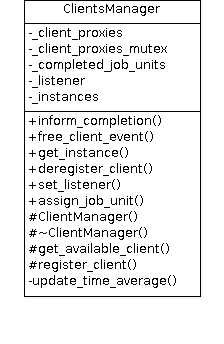
\includegraphics[scale=0.65]{images/ClientsManager-orig.png}
			\caption{Diseño original de la clase \texttt{ClientsManager}}
			\label{fig:ClientsManager:orig}
		\end{center}
	\end{minipage}
	\hfill
	\begin{minipage}[t]{.4\textwidth}
		\begin{center}
	  		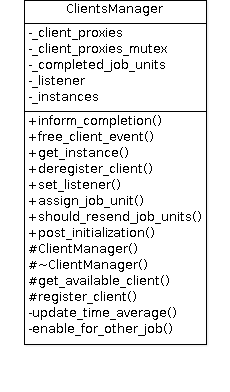
\includegraphics[scale=0.65]{images/ClientsManager-actual.png}
			\caption{Diseño actual de la clase \texttt{ClientsManager}}
			\label{fig:ClientsManager:actual}
		\end{center}
	\end{minipage}
	
\end{figure}

La declaración del método dentro de la clase \texttt{ClientsManager} es la siguiente:\\

\texttt{virtual void post\_initialization() \{\};}\\

Al constructor de la clase \texttt{JobManager} (código \ref{listing:fud:jobmanager}) se le agregó la línea 76 en donde puede observarse la invocación al método mencionado.

\begin{lstlisting}[frame=shadowbox, language=C++, numbers=left, xleftmargin=8mm, framexleftmargin=22pt, basicstyle=\scriptsize, numberstyle=\footnotesize, breaklines=true, breakatwhitespace=false, captionpos=b, caption={Código del constructor de la clase \texttt{JobManager}}, label=listing:fud:jobmanager, backgroundcolor=\color{gris}, firstnumber=56, keywordstyle=\color{Blue}]
JobManager::JobManager() :
    _clients_manager(create_clients_manager()),
    _producingJobs(),
    _waitingJobs(),
    _jobQueue(),
    _pendingList(),
    _ids_to_job_map(),
    _current_job_unit_size(10), //yes, hardcoded to begin with.
    _status(kStopped),
    _mutex(),
    _event_queue()
{
    timeval tm;
    gettimeofday(&tm, NULL);

    openlog(``FUD'', NULL, LOG_LOCAL1);
    syslog(LOG_NOTICE, ``Started FuD.'');

    _clients_manager->set_listener(this);

    _clients_manager->post_initialization();
}
\end{lstlisting}

Por último, la reimplementación de este método en \texttt{BoincClientsManager} realiza la registración del cliente invocando a \texttt{boinc\_register\_client()}:

\begin{lstlisting}[frame=shadowbox, language=C++, numbers=left, xleftmargin=8mm, framexleftmargin=22pt, basicstyle=\scriptsize, numberstyle=\footnotesize, breaklines=true, breakatwhitespace=false, captionpos=b, caption={Código del método \texttt{boinc\_register\_client()} de la clase \texttt{BoincClientsManager}}, label=listing:BoincClientsManager:boinc:register:client, backgroundcolor=\color{gris}, firstnumber=66, keywordstyle=\color{Blue}]
void BoincClientsManager::boinc_register_client()
{
    // Init the client_proxy.
    boinc_log_debug(std::string(``Registering BOINC with FuD.''));
    BoincClientProxy * client = new BoincClientProxy();
    client->set_concurrent_jobs(UNLIMITED_JOBS);
    // Register the unique client proxy.
    register_client(client);
}
\end{lstlisting}


\subsection{Reenvío de \texttt{JobUnits} configurable}
\label{seccion:reenvio:jobunits}

	\subsubsection{Problema}
Luego de resolver la sección anterior (\ref{seccion:jobmanager:post:init}) se encontró el siguiente problema: cada \texttt{JobUnit} que necesitaba ser computada era enviada dos veces por FuD por lo que en cada envío la capa de distribución creaba un \texttt{workunit} distinta. El reenvío de tareas por parte de FuD es normal ya que cuando no hay más trabajos para ser enviados, el framework comienza a reenviar aquellas tareas que aún no han sido reportadas por clientes.

Ésto no era necesario ya que el proyecto BOINC se encarga automáticamente de enviar aquellas tareas que aún no han sido reportadas. Además, esta característica particular de FuD agregaba \texttt{workunits} duplicadas en la base de datos del servidor BOINC innecesariamente ya que BOINC, dependiendo de la configuración del proyecto, replica cada \texttt{workunit}.

	\subsubsection{Solución}
La solución planteada fue que cada manejador de clientes deba especificar si el scheduler de FuD debe reenviar o no las tareas que no hayan sido informadas. Ésto permite que cada capa de distribución pueda decidir si deja que el scheduler reenvíe las tareas, si es ella quien brindará el servicio o bien si la característica queda deshabilitada en su totalidad. Para el caso de BOINC esta característica debe ser deshabilitada por el motivo mencionado anteriormente.

Por consiguiente, el método público agregado dentro de la clase \texttt{ClientsManager} en este caso fue el siguiente:\\

\texttt{virtual bool should\_resend\_job\_units() = 0;}\\

Las figuras \ref{fig:ClientsManager:orig} y \ref{fig:ClientsManager:actual} muestran el diseño original y actual de la clase \texttt{ClientsManager}. En las figuras considerar únicamente el método should\_resend\_job\_units() ya que el resto de las operaciones agregadas no forman parte de esta solución.

Una vez hecho ésto se debió reimplementar el método \texttt{handle\_free\_client\_event()} de la clase \texttt{JobManager} de la capa L2 de FuD para que consulte si se deben reenviar los trabajos. 

El código \ref{listing:jobmanager:handle:free:client} muestra una parte de la implementación de dicho modo. Las líneas 172, 173 y 185 fueron las agregadas para resolver el problema. 
\newpage
\begin{lstlisting}[frame=shadowbox, language=C++, numbers=left, xleftmargin=8mm, framexleftmargin=22pt, basicstyle=\scriptsize, numberstyle=\footnotesize, breaklines=true, breakatwhitespace=false, captionpos=b, caption={Parte del código del método \texttt{handle\_free\_client\_event()} de la clase \texttt{JobManager}}, label=listing:jobmanager:handle:free:client, backgroundcolor=\color{gris}, firstnumber=170, tabsize=4, keywordstyle=\color{Blue}]
if (_jobQueue.empty())
{
	if (_clients_manager->should_resend_job_units()) 
	{
		if (! _pendingList.empty())
		{
			if (_clients_manager->assign_job_unit(*_pendingList.front()))
			{
				//send this one to the back, act as Round Robin
				_pendingList.push_back(_pendingList.front());
				_pendingList.pop_front();
			}
			else
			syslog(LOG_NOTICE, ``Error sending JobUnit %u from Pending List to a client.'', _pendingList.front()->get_id());
		}
	}
}
\end{lstlisting}


\subsection{Múltiples \texttt{JobUnits} a clientes}
\label{seccion:multiples:jobunits:clientes}

	\subsubsection{Problema}
Si bien la primera vez que se ejecutó la aplicación Parallel-Clusterer\footnote{\url{http://code.google.com/p/parallel-clusterer/}} sobre FuD-BOINC en Linux finalizó correctamente, se advirtió que su desempeño no era el esperado debido a que solo se enviaban dos \texttt{JobUnits} a la vez lo que provocaba que su ejecución fuera excesivamente lenta.

Luego de investigar en detalle cómo era el proceso de asignación de tareas de FuD, se observó que el problema se encontraba relacionado directamente con los eventos administrados por la capa de manejo de trabajos (L2) ya que al iniciar la aplicación se generaban solo dos eventos de este tipo provocados, primero, por la presencia de un \texttt{DistributableJob} listo para producir, y segundo por la registración del único cliente al servidor.

La creación de dichos eventos se generan invocando al método \texttt{free\_client\_event()} de la clase \texttt{JobManager}. Luego, el scheduler de FuD, por cada uno de estos eventos intenta asignar una nueva tarea a aquellos clientes que no se encuentren ocupados. Como el único cliente de esta capa siempre se encuentra disponible, ambas tareas eran asignadas inmediatamente pero se debía esperar a que alguna de ellas finalizara ya que en ese momento es cuando se vuelve a generar un nuevo evento de \textit{cliente libre}. 

Es por ello, que el envío de trabajos no funcionaba como se esperaba debido a que el diseño original de FuD solo permitía que el cliente pueda procesar a lo sumo de a una \texttt{JobUnit} por vez.

	\subsubsection{Solución}
La solución que permitió eliminar este problema derivó en un rediseño para permitir que los clientes puedan ejecutar múltiples tareas a la vez. Para ello se debió dar soporte a la capa de distribución.

La idea general que resuelve lo planteado consiste en:

\begin{enumerate}
\item permitir que un cliente, en el momento de su creación, pueda configurar la \textit{cantidad máxima} de tareas que puede ejecutar al mismo tiempo;
\item llevar un registro de la \textit{cantidad de tareas} que un cliente se encuentra computando en un determinado momento. Con cada asignación de tarea este valor será incrementado y con cada informe de resultado será decrementado;
\item determinar si un cliente se encuentra disponible para computar otra tarea basándose de los valores configurados en los dos puntos anteriores;
\item si el cliente no llegó al límite de su capacidad configurada en el punto 1, generar un nuevo evento de \textit{cliente libre}.
\end{enumerate}

A continuación se detalla cada cambio realizado en las clases \texttt{ClientProxy} y \texttt{ClientsManager} en el orden mencionado:

\texttt{\\ClientProxy}:\\

Del diseño original de la clase \texttt{ClientProxy} (\ref{fig:ClientProxy:orig}) se \textit{\textbf{modificaron}} las siguientes operaciones:
\begin{itemize}
\item \texttt{process()}: se cambió su visibilidad pública a protegida manteniendo su prototipo original:\\
\texttt{virtual void process(const JobUnit\& job\_unit) = 0;}

\item \texttt{i\_am\_free()}: el método fue eliminado y reemplazado por \texttt{finish\_one\_job()}.

\item \texttt{busy()}: el método fue eliminado y reemplazado por \texttt{send\_me\_job()}.
\end{itemize}

Al diseño original de la clase \texttt{ClientProxy} (\ref{fig:ClientProxy:orig}) se \textit{\textbf{agregaron}} los siguientes atributos y métodos:

\begin{itemize}
\item \texttt{finish\_one\_job()}: encargado de generar un evento de \textit{cliente libre} y de decrementar a \texttt{\_current\_concurrent\_jobs}. Este método es invocado cuando una tarea es terminada. Su prototipo es:\\
\texttt{void finish\_one\_job();}

\item \texttt{send\_me\_job()}: comprueba si el cliente puede procesar otra tarea en simultáneo o bien si se encuentra ocupado. Su prototipo es:\\
\texttt{bool send\_me\_job() const}

\item \texttt{send\_to\_process()}: se encarga de enviar la \texttt{JobUnit} invocando al método \texttt{process()} y de incrementar a \texttt{\_current\_concurrent\_jobs}. Su prototipo es:\\
\texttt{void send\_to\_process(const JobUnit\& job\_unit);}

\item \texttt{\_concurrent\_jobs}: atributo de la clase que indica el total de tareas en simultáneo que puede computar el cliente. El valor 0 indica que el cliente puede procesar un número ilimitado de tareas en simultáneo (diseñado para BOINC). La constante \texttt{UNLIMITED\_JOBS} representa a dicho valor.

\item \texttt{\_current\_concurrent\_jobs}: atributo de la clase que indica la cantidad de tareas en simultáneo que está computando el cliente en un momento determinado.
\end{itemize}

\begin{figure}[H]
	\hfill
	\begin{minipage}[t]{.4\textwidth}
		\begin{center}
	  		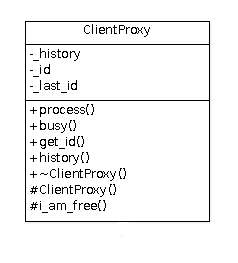
\includegraphics[scale=0.65]{images/ClientProxy-orig.png}
			\caption{Diseño original de la clase \texttt{ClientProxy}}
			\label{fig:ClientProxy:orig}
		\end{center}
	\end{minipage}
	\hfill
	\begin{minipage}[t]{.4\textwidth}
		\begin{center}
	  		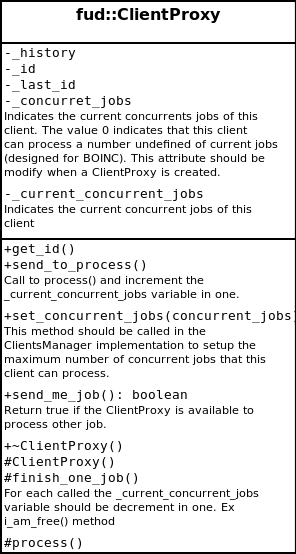
\includegraphics[scale=0.55]{redesing-multiplesJobs-on-client/ClientProxy.png}
			\caption{Diseño actual de la clase \texttt{ClientProxy}}
			\label{fig:ClientProxy:actual}
		\end{center}
	\end{minipage}
\end{figure}

\texttt{\\ClientsManager}:\\

Del diseño original de la clase \texttt{ClientsManager} (\ref{fig:ClientsManager:orig}) se \textbf{agregó} un nuevo método privado encargado de generar un evento en aquellos casos en que el cliente pueda procesar otra \texttt{JobUnit} de manera simultánea. El prototipo de esta operación se define como:

\begin{lstlisting}[frame=shadowbox, language=C++, numbers=left, xleftmargin=8mm, framexleftmargin=22pt, basicstyle=\scriptsize, numberstyle=\footnotesize, breaklines=true, breakatwhitespace=false, captionpos=b, caption={Método \texttt{enable\_for\_other\_job()} de la clase \texttt{ClientsManager}}, label=listing:clientsmanager:enable:for:other:job, backgroundcolor=\color{gris}, firstnumber=129, keywordstyle=\color{Blue}]
void ClientsManager::enable_for_other_job(const ClientProxy* client)
{
    if (client->send_me_job())
        free_client_event(); // It generates a new event
}
\end{lstlisting}

En cuanto a la implementación original de esta clase se hicieron reimplementaciones en dos de sus métodos:

\begin{itemize}
\item \texttt{assign\_job\_unit()}: el código \ref{listing:clientsmanager:assign:job} muestra el cambio realizado. Aquí, se reemplazó la línea 94 por las líneas 95 y 96. Notar que la línea 94 se incluye a modo ilustrativo para indicar cuál fue el código reemplazado.
\begin{lstlisting}[frame=shadowbox, language=C++, numbers=left, xleftmargin=8mm, framexleftmargin=22pt, basicstyle=\scriptsize, numberstyle=\footnotesize, breaklines=true, breakatwhitespace=false, captionpos=b, caption={Método \texttt{assign\_job\_unit()} de la clase \texttt{ClientsManager}}, label=listing:clientsmanager:assign:job, backgroundcolor=\color{gris}, firstnumber=89, tabsize=4]
bool ClientsManager::assign_job_unit(const JobUnit& job_unit)
{
    ClientProxy* client(get_available_client());
    if (client != NULL)
    {
    	// client->process(job_unit);
        client->send_to_process(job_unit); //on the same thread, works asynchronously
        enable_for_other_job(client);
        return true;
    }
    else
    {
        syslog(LOG_NOTICE, ``There are no clients available.'');
        return false;
    }
}
\end{lstlisting}
\item \texttt{get\_available\_client()}: el único cambio realizado aquí fue reemplazar el \texttt{bind} al método \texttt{busy()} por el nuevo método \texttt{send\_me\_job()}. El código original de la línea 114 del código \ref{listing:clientsmanager:get:available:client} era:\\

\texttt{it = find\_if(\_client\_proxies.begin(), \_client\_proxies.end(), !boost::bind(\&ClientProxy::busy, \_1));}
\newpage
\begin{lstlisting}[frame=shadowbox, language=C++, numbers=left, xleftmargin=8mm, framexleftmargin=22pt, basicstyle=\scriptsize, numberstyle=\footnotesize, breaklines=true, breakatwhitespace=false, captionpos=b, caption={Método \texttt{get\_available\_client()} de la clase \texttt{ClientsManager}}, label=listing:clientsmanager:get:available:client, backgroundcolor=\color{gris}, firstnumber=105, tabsize=4, keywordstyle=\color{Blue}]
ClientProxy* ClientsManager::get_available_client()
{
    boost::mutex::scoped_lock glock(_client_proxies_mutex);
    if (_client_proxies.size() == 0)
        return NULL;
    else
    {
        std::list<ClientProxy *>::iterator it;

        it = find_if(_client_proxies.begin(), _client_proxies.end(),
                     boost::bind(&ClientProxy::send_me_job, _1));

        if (it != _client_proxies.end())
        {
            ClientProxy* result(*it);
            _client_proxies.erase(it);
            _client_proxies.push_back(result);
            return result;
        }
        else
            return NULL;
    }
}
\end{lstlisting}
\end{itemize}

Por último, en lo que respecta a la implementación de la capa de distribución de este proyecto, se tuvo que añadir la línea 71 en el método \texttt{register\_client()} (\ref{listing:BoincClientsManager:register:client}) para indicar que el \texttt{ClientProxy} no cuenta con restricciones sobre la cantidad de tareas que puede ejecutar simultáneamente. Ésto fue pensado de esta manera para que todas las \texttt{JobUnits} se traduzcan inmediatamente a \texttt{workunits} de BOINC para que puedan ser rápidamente distribuidas.

A continuación, la figura \ref{fig:rediseno:diagram:seq:mult:jobs} describe el funcionamiento de este rediseño bajo un simple escenario pensado para ilustrar la secuencia de mensajes que interactúan en el envío, recepción y computación de trabajos. Es importante destacar que en el escenario descripto en la figura \ref{fig:rediseno:diagram:seq:mult:jobs}, en una primera instancia solo se envían dos tareas al cliente y que la tercer tarea no es enviada inmediatamente ya que el cliente puede computar como máximo solo dos tareas a la vez. Por cuestiones de simplicidad y lectura del diagrama se omite el envió de la tercer tarea una vez que se reporta el primer resultado.

\begin{figure}[H]
	\begin{center}
  		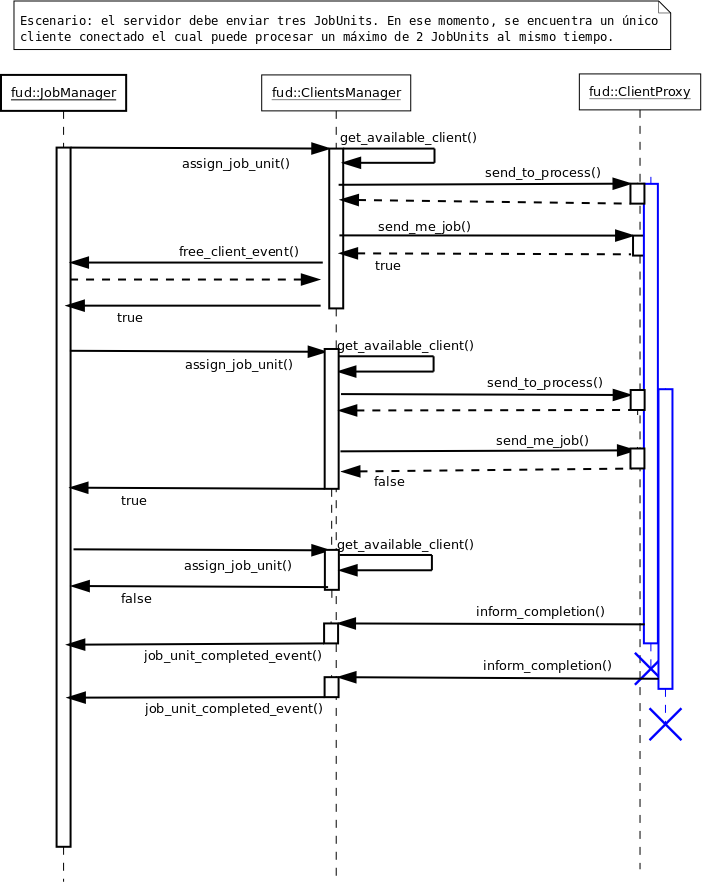
\includegraphics[scale=0.42]{redesing-multiplesJobs-on-client/assign_job_unit_seq_diagram.png}
		\caption{Diagrama de secuencia del rediseño de múltiples JobUnits a clientes}
		\label{fig:rediseno:diagram:seq:mult:jobs}
	\end{center}
\end{figure}


\newpage
\section{Métricas de código}

FuD-BOINC fue implementado en \texttt{7} archivos fuente los cuales suman un total de \texttt{1243} líneas de texto entre las que se distinguen líneas en blanco, comentarios y líneas de código. La tabla \ref{metrics:cloc} muestra un resumen de los resultados obtenidos al correr la aplicación \textit{Cloc} sobre los archivos de implementación de FuD-BOINC.

\begin{table}[!htf]
    \begin{center}
    \begin{tabular}{|l|r|r|r|r|c|}
    \hline
    \multicolumn{2}{|c|}{Files} & \multicolumn{3}{|c|}{Line Types} & \hspace{0.2cm}\% \\
    \hline
    \textbf{Type} & \textbf{Count} & \textbf{Blank} & \textbf{Comment} & \textbf{Source} & \small{\textbf{\#Comms./Tot.}}\\
    \hline
    \texttt{C++ source} & 2 &  130  &  120  &   466  &   20,47\\
    \hline
    \texttt{C++ header} & 5 &   95  &  292  &   140  &   67,59 \\
    \hline
    \textbf{Total} &    7   &  225  &  412  &   606  &   40,47 \\
    \hline
    \end{tabular}
    \caption{Resultados de CLOC para FuD-BOINC}
    \label{metrics:cloc}
    \end{center}
\end{table}

Podemos observar que de acuerdo a los resultados obtenidos, la capa de distribución FuD-BOINC no es un proyecto de gran tamaño. De un total de \texttt{1243} líneas escritas, sólo \texttt{606} líneas se corresponden a código fuente; un número relativamente bajo comparado con la complejidad del proyecto.

\textit{Dijkstra} escribió un interesante ensayo sobre por qué las industrias de software no deberían considerar las líneas de código como una medida exacta de la productividad del software o del programador. Mientras más líneas de código tenga, mayor es la complejidad de un producto de software, pero en el sentido de que es más difícil de mantener y entender; no tiene una relación directa con la funcionalidad que provee.

Otro resultado sorprendente que podemos observar en la tabla \ref{metrics:cloc} es el número de líneas de comentarios en el proyecto y su porcentaje con respecto al total de líneas de código efectivas del mismo:

$$\frac{\#comment\_lines}{\#comment\_lines + \#code\_lines}$$

Este valor es aproximadamente \texttt{0,40}, lo que indica que el \texttt{40\%} de las líneas de código se corresponden a líneas de comentarios. Este porcentaje se debe a que todos los archivos de implementación, por más chico que sea, poseen un header que ofrece ciertos detalles sobre el mismo, como sus autores, fecha de creación y la licencia por cual se rigen. En el código \ref{listing:fud:header} se puede ver el header que debe poseer cada archivo de código fuente.


\begin{lstlisting}[frame=shadowbox, language=C++, numbers=left, xleftmargin=8mm, framexleftmargin=22pt, basicstyle=\scriptsize, numberstyle=\footnotesize, breaklines=true, breakatwhitespace=false, caption={Header común en los archivos de implementación}, label=listing:fud:header, backgroundcolor=\color{gris}, firstnumber=170, tabsize=4, keywordstyle=\color{Blue}]
/**
*  \file:      boinc_clients_manager.h
*  \brief      Definition of BoincClientsManager class.
*              System:     FuD
*              Language:   C++
*
*  @author     Lucas Besso     -   E-Mail: lbesso AT gmail.com
*  @author     Raul Striglio   -   E-Mail: rulitox.s AT gmail.com
*
*
*  @Last Update:
*      $Id: boinc_clients_manager.h 850 2011-12-12 15:02:09Z lbesso $
*      $URL: https://fud.googlecode.com/svn/branches/boinc/src/middlewares/boinc/server/boinc_clients_manager.h $
*      $LastChangedBy: lbesso $ Author of last commit
*
*
* FuD is free software: you can redistribute it and/or modify
* it under the terms of the GNU General Public License as published by
* the Free Software Foundation, either version 3 of the License, or
* (at your option) any later version.
*
* FuD is distributed in the hope that it will be useful,
* but WITHOUT ANY WARRANTY; without even the implied warranty of
* MERCHANTABILITY or FITNESS FOR A PARTICULAR PURPOSE.  See the
* GNU General Public License for more details.
*
* You should have received a copy of the GNU General Public License
* along with FuD.  If not, see <http://www.gnu.org/licenses/>.
*/
\end{lstlisting}

Otro motivo que explica esta cantidad de líneas de comentarios es que todo componente de software tal como clases, estructuras, funciones, atributos, etc., tiene una descripción detallada a ser interpretada por Doxygen para la generación de automática de documentos. En el código \ref{listing:fud:doxygen} podemos observar un ejemplo de notación utilizando \texttt{doxygen}\footnote{\url{http://www.doxygen.org/}}.

\begin{lstlisting}[frame=shadowbox, language=C++, numbers=left, xleftmargin=8mm, framexleftmargin=22pt, basicstyle=\scriptsize, numberstyle=\footnotesize, breaklines=true, breakatwhitespace=false, caption={Ejemplo de comentario Doxygen utilizado en FuD-BOINC}, label=listing:fud:doxygen, backgroundcolor=\color{gris}, firstnumber=170, tabsize=4, keywordstyle=\color{Blue}]
            /** 
            * Create the boinc workunit to be computed.
            *
            *   @param name_input_file : The workunit's inputfile name
            *   @param wu_template : The BOINC's workunit template
            */
            void create_boinc_work(std::string name_input_file, const char* wu_template) throw (BoincWorkException);
\end{lstlisting}

En el apéndice \ref{chapter:FuD-BOINC:metrics_report} podemos encontrar un reporte completo sobre las métricas de código generado con la aplicación \texttt{cccc}\footnote{\url{http://cccc.sourceforge.net/}}. Éste incluye varias métricas de diseño orientado a objetos y todo tipo de información relevante en lo que respecta al código.

\subsection{Cobertura de código}

La cobertura de código es una medida utilizada en pruebas de software. Ésta describe el grado en que el código fuente de un programa ha sido testeado. Para FuD-BOINC se ejecutó la prueba de cobertura de código mediante la aplicación \texttt{GCov}\footnote{\url{http://gcc.gnu.org/onlinedocs/gcc/Gcov.html}}.

En la tabla \ref{table:gcov:server} se muestra la cobertura de código de los archivos que implementan el lado servidor de FuD-BOINC y en la tabla \ref{table:gcov:client} se muestra la cobertura de código de los archivos que implementan el lado cliente de FuD-BOINC.

\begin{table}[H]
    \begin{center}
    \begin{tabular}{|l|r|r|c|}
        \hline
        & \multicolumn{2}{|c|}{Líneas de código} & Porcentaje \\
        \hline
        \textbf{Archivo} & \textbf{Total} & \textbf{Ejecutado} & \hspace{0.2cm}\textbf{\%} \\
        \hline
        \scriptsize{boinc\_constants.h} & 4 & 4 & 100 \\
        \hline 
        \scriptsize{boinc\_clients\_manager.cpp} & 240 & 163 & 67.9 \\
        \hline 
        \scriptsize{boinc\_client\_manager.h} & 15 & 9 & 60 \\
        \hline 
        \scriptsize{boinc\_exception.h} & 4 & 0 & 0 \\
        \hline 
    \end{tabular}
    \caption{Resultados de cobertura para los archivos de código del servidor FuD-BOINC}
    \label{table:gcov:server}
    \end{center}
\end{table}

\begin{table}[H]
    \begin{center}
    \begin{tabular}{|l|r|r|c|}
        \hline
        & \multicolumn{2}{|c|}{Líneas de código} & Porcentaje \\
        \hline
        \textbf{Archivo} & \textbf{Total} & \textbf{Ejecutado} & \hspace{0.2cm}\textbf{\%} \\
        \hline
        \scriptsize{boinc\_distribution.h} & 1 & 0 & 0.00 \\
        \hline 
        \scriptsize{boinc\_distribution.cpp} & 240 & 163 & 67.9 \\
        \hline 
        \scriptsize{boinc\_client\_manager.h} & 58 & 43,99 & 75.86 \\
        \hline 
        \scriptsize{boinc\_exception.h} & 2 & 0 & 0 \\
        \hline 
    \end{tabular}
    \caption{Resultados de cobertura para los archivos de código del cliente FuD-BOINC}
    \label{table:gcov:client}
    \end{center}
\end{table}

